% Template adapted from https://github.com/jgm/pandoc-templates/blob/master/default.latex
% To be used with XeLaTex in memoiR
%%%%%%%%%%%%%%%%%%%%%%%%%%%%%%%%%%%%%%%%%%%%%%%%%%%%%%%%%%%%%%%%%%%%%%%%%%%%%%%%%%%%%%%%%

% Options for packages loaded elsewhere
\PassOptionsToPackage{unicode=true}{hyperref}
\PassOptionsToPackage{hyphens}{url}
\PassOptionsToPackage{dvipsnames,svgnames*,x11names*}{xcolor}
% Right to left support


\documentclass[
  10pt,
  italian,
  a4paper,
  extrafontsizes,onecolumn,openright
  ]{memoir}

% Double (or whatever) spacing

% Math
\usepackage{amssymb, amsmath}
% mathspec: arbitrary math fonts
\usepackage{unicode-math}
\defaultfontfeatures{Scale=MatchLowercase}
\defaultfontfeatures[\rmfamily]{Ligatures=TeX,Scale=1}

% Fonts
\usepackage{lmodern}
\usepackage{fontspec}

% Main font
% Specific sanserif font
% Specific monotype font
\setmonofont[Scale=0.85]{Inconsolata}
% Specific math font
% Chinese, Japanese, Corean fonts

% Use upquote for straight quotes in verbatim environments
\usepackage{upquote}
% Use microtype
\usepackage[]{microtype}
\UseMicrotypeSet[protrusion]{basicmath} % disable protrusion for tt fonts

% Verbatim in note

% Color links
\usepackage{xcolor}

% Strikeout

% Necessary for code chunks

% Listings package

% Tables
\usepackage{longtable,booktabs,tabu}
% Fix footnotes in tables (requires footnote package)
\IfFileExists{footnote.sty}{\usepackage{footnote}\makesavenoteenv{longtable}}{}

% Graphics
\usepackage{graphicx,grffile}
\graphicspath{{images/}}
\makeatletter
\def\maxwidth{\ifdim\Gin@nat@width>\linewidth\linewidth\else\Gin@nat@width\fi}
\def\maxheight{\ifdim\Gin@nat@height>\textheight\textheight\else\Gin@nat@height\fi}
\makeatother
% Scale images if necessary, so that they will not overflow the page
% margins by default, and it is still possible to overwrite the defaults
% using explicit options in \includegraphics[width, height, ...]{}
\setkeys{Gin}{width=\maxwidth,height=\maxheight,keepaspectratio}

% Prevent overfull lines
\setlength{\emergencystretch}{3em}  
\providecommand{\tightlist}{%
  \setlength{\itemsep}{0pt}\setlength{\parskip}{0pt}}

% Number sections for memoir (secnumdepth counter is ignored)
\setsecnumdepth{section}

% Set default figure placement to htbp
\makeatletter
\def\fps@figure{htbp}
\makeatother

% Spacing in lists
\usepackage{enumitem}

% Polyglossia
\usepackage{polyglossia}
\setmainlanguage{it}
\setotherlanguage{en-US}

% BibLaTeX
\usepackage[backend=biber,style=authoryear-ibid,isbn=false,backref=true,giveninits=true,uniquename=init,maxcitenames=2,maxbibnames=150,sorting=nyt,sortcites=false,style=apa]{biblatex}
\addbibresource{refs.bib}

% cslreferences environment required by pandoc > 2.7



%%%%%%%%%%%%%%%%%%%%%%%%%%%%%%%%%%%%%%%%%%%%%%%%%%%%%%%%%%
% memoiR format

% Chapter Summary environment 
\usepackage[tikz]{bclogo}
\newenvironment{Summary}
  {\begin{bclogo}[logo=\bctrombone, noborder=true, couleur=lightgray!50]{In breve}\parindent0pt}
  {\end{bclogo}}
% Syntax:
%
%```{block, type='Summary'}
% Deliver message here.
% ```

% scriptsize code 
\let\oldverbatim\verbatim
\def\verbatim{\oldverbatim\scriptsize}
% Applies to code blocks and R code results
% code chunk options size='scriptsize' applies only to R code and results
% if the code chunk sets a different size, \def\verbatim{...} is prioritary for code results 


% Layout
%%%%%%%%%%%%%%%%%%%%%%%%%%%%%%%%%%%%%%%%%%%%%%%%%%%%%%%%%%

% Based on memoir, style companion
\newcommand{\MemoirChapStyle}{daleif1}
\newcommand{\MemoirPageStyle}{Ruled}

% Space between paragraphs
\usepackage{parskip}
  \abnormalparskip{3pt}

% Adjust margin paragraphs vertical position
\usepackage{marginfix}


% Margins
%%%%%%%%%%%%%%%%%%%%%%%%%%%%%%%%%%%%%%%

% allow use of '-',+','/' ans '*' to make simple length computation
\usepackage{calc}

% Full-width figures utilities
\newlength\widthw % full width
\newlength{\rf}
\newcommand*{\definesHSpace}{
  \strictpagecheck % slower but efficient detection of odd/even pages
  \checkoddpage
  \ifoddpage
  \setlength{\rf}{0mm}
  \else
  \setlength{\rf}{\marginparsep+\marginparwidth}
  \fi
}

\makeatletter
% 1" margins for the front matter.
\newcommand*{\SmallMargins}{
  \setlrmarginsandblock{1.5in}{1.5in}{*}
  \setmarginnotes{0.1in}{0.1in}{0.1in}
 \setulmarginsandblock{1.5in}{1in}{*}
  \checkandfixthelayout
  \ch@ngetext
  \clearpage
  \setlength{\widthw}{\textwidth+\marginparsep+\marginparwidth}
  \footnotesatfoot
  \chapterstyle{\MemoirChapStyle}  % Chapter and page styles must be recalled
  \pagestyle{\MemoirPageStyle}
}

% 3" outer margin for the main matter
\newcommand{\LargeMargins}{\SmallMargins}
\makeatother

% Figure captions and footnotes in outer margins


% Main title page with filigrane
%%%%%%%%%%%%%%%%%%%%%%%%%%%%%%%%%%%%%%%%%%%%%%%%%%%%%%%%%%

% Text blocks
\usepackage[absolute,overlay]{textpos}
  \setlength{\TPHorizModule}{1mm}
  \setlength{\TPVertModule}{1mm}

\newcommand{\MainTitlePage}[2]{
  \SmallMargins % Margins
  \pagestyle{empty} % No header/footer
  \textblockorigin{\stockwidth-\paperwidth-\trimedge}{\trimtop} % recto
  \begin{textblock*}{2mm}(\spinemargin/2,\uppermargin/2)
    \rule{1pt}{\paperheight-\uppermargin}
  \end{textblock*}
  \begin{textblock*}{\paperwidth*2/3}(\paperwidth/5, \paperheight/5)
    \flushright
    \begin{Spacing}{3}
      {\fontfamily{qtm}\selectfont\fontsize{45}{45}\selectfont\textsc{\thetitle}}
    \end{Spacing}
  \end{textblock*}
    \begin{textblock*}{\paperwidth*2/3}(\paperwidth/5, \paperheight/2)
    \flushright
    {\fontfamily{qtm}\huge\theauthor}
  \end{textblock*}
    \begin{textblock*}{\paperwidth*2/3}[0, 1](\spinemargin, \uppermargin+\textheight)
    \normalfont\thedate
  \end{textblock*}
  ~\\ % Print a character or the page will not exist
  \newpage
  \textblockorigin{\trimedge}{\trimtop} % verso
  \begin{textblock*}{\textwidth}(\paperwidth-\spinemargin-\textwidth, \uppermargin)
    #1
  \end{textblock*}
  \begin{textblock*}{\textwidth}[0,1](\paperwidth-\spinemargin-\textwidth, \uppermargin+\textheight+\footskip)
    \centering
    
\includegraphics[width=\paperwidth/4]{logo}\\ \bigskip
    #2
  \end{textblock*}
  ~\\ % Print a character or the page will not exist
  \newpage
}

% Clear page and open an even one (\clearpage opens an odd one)
\newcommand{\evenpage}{
  \clearpage
  \strictpagecheck % slower but efficient detection of odd/even pages
  \checkoddpage
  \ifoddpage
    \thispagestyle{empty}
    ~\\ % Print a character or the page will not exist
    \newpage
  \else
    % do nothing
  \fi
}


%% PDF title page to insert
%%%%%%%%%%%%%%%%%%%%%%%%%%%%%%%%%%%%%%%%%%%%%%%%%%%%%%%%%%



%% Bibliography
%%%%%%%%%%%%%%%%%%%%%%%%%%%%%%%%%%%%%%%%%%%%%%%%%%%%%%%%%%

\usepackage[strict,autostyle]{csquotes}
% Repeated citation as author-year-title instead of author-title (modification of footcite:note in verbose-inote.cbx)

%% Table of Contents
%%%%%%%%%%%%%%%%%%%%%%%%%%%%%%%%%%%%%%%%%%%%%%%%%%%%%%%%%%

% fix the typesetting of the part number
\renewcommand\partnumberlinebox[2]{#2\ ---\ }


% Fonts
%%%%%%%%%%%%%%%%%%%%%%%%%%%%%%%%%%%%%%%%%%%%%%%%%%%%%%%%%%


% Hyperref comes last
%%%%%%%%%%%%%%%%%%%%%%%%%%%%%%%%%%%%%%%%%%%%%%%%%%%%%%%%%%

\usepackage{hyperref}
\hypersetup{
  pdftitle={Psicometria},
  pdfauthor={Corrado Caudek},
  colorlinks=true,
  linkcolor=Maroon,
  citecolor=Blue,
  urlcolor=Blue,
  breaklinks=true}

% Don't use monospace font for urls
\urlstyle{same}


% Title, author, date from YAML to LaTeX
%%%%%%%%%%%%%%%%%%%%%%%%%%%%%%%%%%%%%%%%%%%%%%%%%%%%%%%%%%

\title{Psicometria}

\author{Corrado Caudek}

\date{2021-11-11}


% Include headers (preamble.tex) here
%%%%%%%%%%%%%%%%%%%%%%%%%%%%%%%%%%%%%%%%%%%%%%%%%%%%%%%%%%
% Add LaTeX code into the preamble of the document here
\hyphenation{bio-di-ver-si-ty sap-lings}


%%%%%%%%%%%%%%%%%%%%%%%%%%%%%%%%%%%%%%%%%%%%%%%%%%%%%%%%%%%%%%%%%%%%%%%%%
% memoiR dalef3 chapter style 
% https://ctan.crest.fr/tex-archive/info/latex-samples/MemoirChapStyles/MemoirChapStyles.pdf
\usepackage{soul}
\definecolor{nicered}{rgb}{.647,.129,.149}
\makeatletter
\newlength\dlf@normtxtw
\setlength\dlf@normtxtw{\textwidth}
\def\myhelvetfont{\def\sfdefault{mdput}}
\newsavebox{\feline@chapter}
\newcommand\feline@chapter@marker[1][4cm]{%
  \sbox\feline@chapter{%
    \resizebox{!}{#1}{\fboxsep=1pt%
	  \colorbox{nicered}{\color{white}\bfseries\sffamily\thechapter}%
	}}%
  \rotatebox{90}{%
    \resizebox{%
	  \heightof{\usebox{\feline@chapter}}+\depthof{\usebox{\feline@chapter}}}%
	{!}{\scshape\so\@chapapp}}\quad%
  \raisebox{\depthof{\usebox{\feline@chapter}}}{\usebox{\feline@chapter}}%
 }
\newcommand\feline@chm[1][4cm]{%
  \sbox\feline@chapter{\feline@chapter@marker[#1]}%
  \makebox[0pt][l]{% aka \rlap
    \makebox[1cm][r]{\usebox\feline@chapter}%
  }}
\makechapterstyle{daleif1}{
  \renewcommand\chapnamefont{\normalfont\Large\scshape\raggedleft\so}
  \renewcommand\chaptitlefont{\normalfont\huge\bfseries\scshape\color{nicered}}
  \renewcommand\chapternamenum{}
  \renewcommand\printchaptername{}
  \renewcommand\printchapternum{\null\hfill\feline@chm[2.5cm]\par}
  \renewcommand\afterchapternum{\par\vskip\midchapskip}
  \renewcommand\printchaptertitle[1]{\chaptitlefont\raggedleft ##1\par}
}
\makeatother

\DeclareMathOperator{\Var}{Var} % Define variance operator
\DeclareMathOperator{\SD}{SD} % Define sd operator
\DeclareMathOperator{\Cov}{Cov} % Define covariance operator
\DeclareMathOperator{\Corr}{Corr} % Define correlation operator
\DeclareMathOperator{\Me}{Me} % Define mediane operator
\DeclareMathOperator{\Mo}{Mo} % Define mode operator
\DeclareMathOperator{\Bin}{Bin} % Define binomial operator
\DeclareMathOperator{\Bernoulli}{Bernoulli} % Define Bernoulli operator
\DeclareMathOperator{\Poi}{Poi} % Define Poisson operator
\DeclareMathOperator{\Uniform}{Uniform} % Define Uniform operator
\DeclareMathOperator{\Cauchy}{Cauchy} % Define Cauchy operator
\DeclareMathOperator{\elpd}{elpd} % Define elpd operator
\DeclareMathOperator{\lppd}{lppd} % Define lppd operator
\DeclareMathOperator{\LOO}{LOO} % Define LOO operator
\DeclareMathOperator{\B}{\mathscr{B}} % Define Bernoulli operator
\newcommand{\R}{\textsf{R}} % Define R programming language symbol
\newcommand{\E}{\mathbb{E}} % Define expected value operator
\newcommand{\Real}{\mathbb{R}} % Define real number operator
\newcommand{\Prob}{\mathscr{P}}
\DeclareMathOperator*{\argmin}{arg\,min} % thin space, limits on side in displays
\DeclareMathOperator*{\argmax}{arg\,max} % thin space, limits on side in displays

\raggedbottom % allow variable (ragged) site heights
\frenchspacing

\usepackage[
  labelfont=bf, 
  font={small, it} 
]{caption} 
\usepackage{upquote} % print correct quotes in verbatim-environments
\usepackage{empheq} 
\usepackage{xfrac}




\usepackage{booktabs}
\usepackage{longtable}
\usepackage{array}
\usepackage{multirow}
\usepackage{wrapfig}
\usepackage{float}
\usepackage{colortbl}
\usepackage{pdflscape}
\usepackage{tabu}
\usepackage{threeparttable}
\usepackage{threeparttablex}
\usepackage[normalem]{ulem}
\usepackage{makecell}
\usepackage{xcolor}


% End of preamble
%%%%%%%%%%%%%%%%%%%%%%%%%%%%%%%%%%%%%%%%%%%%%%%%%%%%%%%%%%


\begin{document}
\frontmatter

% Title page
%%%%%%%%%%%%%%%%%%%%%%%%%%%%%%%%%%%%%%%%%%%%%%%%%%%%%%%%%%


\MainTitlePage{Questo documento è stato realizzato con:

\begin{itemize}
  \item \LaTeX\; e la classe memoir (\url{http://www.ctan.org/pkg/memoir});
  \item $\R$ (\url{http://www.r-project.org/}) e RStudio (\url{http://www.rstudio.com/});
  \item bookdown (\url{http://bookdown.org/}) e memoiR (\url{https://ericmarcon.github.io/memoiR/}).
\end{itemize}}{Nel blog della mia pagina personale sono forniti alcuni approfondimenti degli argomenti qui trattati.

\url{https://ccaudek.github.io/caudeklab/}}


% Before Body
%%%%%%%%%%%%%%%%%%%%%%%%%%%%%%%%%%%%%%%%%%%%%%%%%%%%%%%%%%





% Contents
%%%%%%%%%%%%%%%%%%%%%%%%%%%%%%%%%%%%%%%%%%%%%%%%%%%%%%%%%%

\LargeMargins
{
\hypersetup{linkcolor=}
\setcounter{tocdepth}{2}
\tableofcontents
}


% Body
%%%%%%%%%%%%%%%%%%%%%%%%%%%%%%%%%%%%%%%%%%%%%%%%%%%%%%%%%%

\LargeMargins
\scriptsize

\normalsize

\chapter*{}

\vfill

\scriptsize

\normalsize

\scriptsize

Copyright \(\copyright\) 2022.

\normalsize

Data della versione presente: Novembre 11, 2021.

\hypertarget{prefazione}{%
\chapter{Prefazione}\label{prefazione}}

\textbf{Data Science per psicologi} contiene il materiale delle lezioni dell'insegnamento di \emph{Psicometria B000286} (A.A. 2021/2022) rivolto agli studenti del primo anno del Corso di Laurea in Scienze e Tecniche Psicologiche dell'Università degli Studi di Firenze.

L'insegnamento di Psicometria si propone di fornire agli studenti un'introduzione all'analisi dei dati in psicologia.
Le conoscenze/competenze che verranno sviluppate in questo insegnamento sono quelle della \emph{Data science}, ovvero le conoscenze/competenze che si pongono all'intersezione tra statistica (ovvero, richiedono la capacità di comprendere teoremi statistici) e informatica (ovvero, richiedono la capacità di sapere utilizzare un software).

\hypertarget{la-psicologia-e-la-data-science}{%
\section*{La psicologia e la Data Science}\label{la-psicologia-e-la-data-science}}
\addcontentsline{toc}{section}{La psicologia e la Data Science}

\begin{quote}
It's worth noting, before getting started, that this material is hard. If you find yourself confused at any point, you are normal. Any sense of confusion you feel is just your brain correctly calibrating to the subject matter. Over time, confusion is replaced by comprehension {[}\ldots{]} --- Richard McElreath
\end{quote}

Sembra sensato spendere due parole su un tema che è importante per gli studenti: quello indicato dal titolo di questo Capitolo. È ovvio che agli studenti di psicologia la statistica non piace. Se piacesse, forse studierebbero Data Science e non psicologia; ma non lo fanno. Di conseguenza, gli studenti di psicologia si chiedono: ``perché dobbiamo perdere tanto tempo a studiare queste cose quando in realtà quello che ci interessa è tutt'altro?'\,' Questa è una bella domanda.

C'è una ragione molto semplice che dovrebbe farci capire perché la Data Science è così importante per la psicologia. Infatti, a ben pensarci, la psicologia è una disciplina intrinsecamente statistica, se per statistica intendiamo quella disciplina che studia la variazione delle caratteristiche degli individui nella popolazione. La psicologia studia \emph{gli individui} ed è proprio la variabilità inter- e intra-individuale ciò che vogliamo descrivere e, in certi casi, predire. In questo senso, la psicologia è molto diversa dall'ingegneria, per esempio. Le proprietà di un determinato ponte sotto certe condizioni, ad esempio, sono molto simili a quelle di un altro ponte, sotto le medesime condizioni. Quindi, per un ingegnere la statistica è poco importante: le proprietà dei materiali sono unicamente dipendenti dalla loro composizione e restano costanti. Ma lo stesso non può dirsi degli individui: ogni individuo è unico e cambia nel tempo. E le variazioni tra gli individui, e di un individuo nel tempo, sono l'oggetto di studio proprio della psicologia: è dunque chiaro che i problemi che la psicologia si pone sono molto diversi da quelli affrontati, per esempio, dagli ingegneri. Questa è la ragione per cui abbiamo tanto bisogno della \emph{data science} in psicologia: perché la \emph{data science} ci consente di descrivere la variazione e il cambiamento. E queste sono appunto le caratteristiche di base dei fenomeni psicologici.

Sono sicuro che, leggendo queste righe, a molti studenti sarà venuta in mente la seguente domanda: perché non chiediamo a qualche esperto di fare il ``lavoro sporco'' (ovvero le analisi statistiche) per noi, mentre noi (gli psicologi) ci occupiamo solo di ciò che ci interessa, ovvero dei problemi psicologici slegati dai dettagli ``tecnici'' della \emph{data science}?
La risposta a questa domanda è che non è possibile progettare uno studio psicologico sensato senza avere almeno una comprensione rudimentale della \emph{data science}. Le tematiche della \emph{data science} non possono essere ignorate né dai ricercatori in psicologia né da coloro che svolgono la professione di psicologo al di fuori dell'Università. Infatti, anche i professionisti al di fuori dall'università non possono fare a meno di leggere la letteratura psicologica più recente: il continuo aggiornamento delle conoscenze è infatti richiesto dalla deontologia della professione. Ma per potere fare questo è necessario conoscere un bel po' di \emph{data science}! Basta aprire a caso una rivista specialistica di psicologia per rendersi conto di quanto ciò sia vero: gli articoli che riportano i risultati delle ricerche psicologiche sono zeppi di analisi statistiche e di modelli formali. E la comprensione della letteratura psicologica rappresenta un requisito minimo nel bagaglio professionale dello psicologo.

Le considerazioni precedenti cercano di chiarire il seguente punto: la \emph{data science} non è qualcosa da studiare a malincuore, in un singolo insegnamento universitario, per poi poterla tranquillamente dimenticare. Nel bene e nel male, gli psicologi usano gli strumenti della \emph{data science} in tantissimi ambiti della loro attività professionale: in particolare quando costruiscono, somministrano e interpretano i test psicometrici. È dunque chiaro che possedere delle solide basi di \emph{data science} è un tassello imprescindibile del bagaglio professionale dello psicologo. In questo insegnamento verrano trattati i temi base della \emph{data science} e verrà adottato un punto di vista bayesiano, che corrisponde all'approccio più recente e sempre più diffuso in psicologia.

\hypertarget{come-studiare}{%
\section*{Come studiare}\label{come-studiare}}
\addcontentsline{toc}{section}{Come studiare}

\begin{quote}
I know quite certainly that I myself have no special talent. Curiosity, obsession and dogged endurance, combined with self-criticism, have brought me to my ideas. --- Albert Einstein
\end{quote}

Il giusto metodo di studio per prepararsi all'esame di Psicometria è quello di seguire attivamente le lezioni, assimilare i concetti via via che essi vengono presentati e verificare in autonomia le procedure presentate a lezione. Incoraggio gli studenti a farmi domande per chiarire ciò che non è stato capito appieno. Incoraggio gli studenti a utilizzare i forum attivi su Moodle e, soprattutto, a svolgere gli esercizi proposti su Moodle. I problemi forniti su Moodle rappresentano il livello di difficoltà richiesto per superare l'esame e consentono allo studente di comprendere se le competenze sviluppate fino a quel punto sono sufficienti rispetto alle richieste dell'esame.

La prima fase dello studio, che è sicuramente individuale, è quella in cui è necessario acquisire le conoscenze teoriche relative ai problemi che saranno presentati all'esame. La seconda fase di studio, che può essere facilitata da scambi con altri e da incontri di gruppo, porta ad acquisire la capacità di applicare le conoscenze: è necessario capire come usare un software (\R) per applicare i concetti statistici alla specifica situazione del problema che si vuole risolvere. Le due fasi non sono però separate: il saper fare molto spesso ci aiuta a capire meglio.

\hypertarget{sviluppare-un-metodo-di-studio-efficace}{%
\section*{Sviluppare un metodo di studio efficace}\label{sviluppare-un-metodo-di-studio-efficace}}
\addcontentsline{toc}{section}{Sviluppare un metodo di studio efficace}

\begin{quote}
Memorization is not learning. --- Richard Phillips Feynman
\end{quote}

Avendo insegnato molte volte in passato un corso introduttivo di analisi dei dati ho notato nel corso degli anni che gli studenti con l'atteggiamento mentale che descriverò qui sotto generalmente ottengono ottimi risultati. Alcuni studenti sviluppano naturalmente questo approccio allo studio, ma altri hanno bisogno di fare uno sforzo per maturarlo. Fornisco qui sotto una breve descrizione del ``metodo di studio'\,' che, nella mia esperienza, è il più efficace per affrontare le richieste di questo insegnamento \autocite{burger20125}.

\begin{itemize}
\tightlist
\item
  Dedicate un tempo sufficiente al materiale di base, apparentemente facile; assicuratevi di averlo capito bene. Cercate le lacune nella vostra comprensione. Leggere presentazioni diverse dello stesso materiale (in libri o articoli diversi) può fornire nuove intuizioni.
\end{itemize}

\begin{itemize}
\item
  Gli errori che facciamo sono i nostri migliori maestri. Istintivamente cerchiamo di dimenticare subito i nostri errori. Ma il miglior modo di imparare è apprendere dagli errori che commettiamo. In questo senso, una soluzione corretta è meno utile di una soluzione sbagliata. Quando commettiamo un errore questo ci fornisce un'informazione importante: ci fa capire qual è il materiale di studio sul quale dobbiamo ritornare e che dobbiamo capire meglio.
\item
  C'è ovviamente un aspetto ``psicologico'' nello studio. Quando un esercizio o problema ci sembra incomprensibile, la cosa migliore da fare è dire: ``mi arrendo'', ``non ho idea di cosa fare!''. Questo ci rilassa: ci siamo già arresi, quindi non abbiamo niente da perdere, non dobbiamo più preoccuparci. Ma non dobbiamo fermarci qui. Le cose ``migliori'' che faccio (se ci sono) le faccio quando non ho voglia di lavorare. Alle volte, quando c'è qualcosa che non so fare e non ho idea di come affontare, mi dico: ``oggi non ho proprio voglia di fare fatica'', non ho voglia di mettermi nello stato mentale per cui ``in 10 minuti devo risolvere il problema perché dopo devo fare altre cose''. Però ho voglia di \emph{divertirmi} con quel problema e allora mi dedico a qualche aspetto ``marginale'' del problema, che so come affrontare, oppure considero l'aspetto più difficile del problema, quello che non so come risolvere, ma invece di cercare di risolverlo, guardo come altre persone hanno affrontato problemi simili, opppure lo stesso problema in un altro contesto. Non mi pongo l'obiettivo ``risolvi il problema in 10 minuti'', ma invece quello di farmi un'idea ``generale'' del problema, o quello di capire un caso più specifico e più semplice del problema. Senza nessuna pressione. Infatti, in quel momento ho deciso di non lavorare (ovvero, di non fare fatica). Va benissimo se ``parto per la tangente'', ovvero se mi metto a leggere del materiale che sembra avere poco a che fare con il problema centrale (le nostre intuizioni e la nostra curiosità solitamente ci indirizzano sulla strada giusta). Quando faccio così, molto spesso trovo la soluzione del problema che mi ero posto e, paradossalmente, la trovo in un tempo minore di quello che, in precedenza, avevo dedicato a ``lavorare'' al problema. Allora perché non faccio sempre così? C'è ovviamente l'aspetto dei ``10 minuti'' che non è sempre facile da dimenticare. Sotto pressione, possiamo solo agire in maniera automatica, ovvero possiamo solo applicare qualcosa che già sappiamo fare. Ma se dobbiamo imparare qualcosa di nuovo, la pressione è un impedimento.
\item
  È utile farsi da soli delle domande sugli argomenti trattati, senza limitarsi a cercare di risolvere gli esercizi che vengono assegnati. Quando studio qualcosa mi viene in mente: ``se questo è vero, allora deve succedere quest'altra cosa''. Allora verifico se questo è vero, di solito con una simulazione. Se i risultati della simulazione sono quelli che mi aspetto, allora vuol dire che ho capito. Se i risultati sono diversi da quelli che mi aspettavo, allora mi rendo conto di non avere capito e ritorno indietro a studiare con più attenzione la teoria che pensavo di avere capito -- e ovviamente mi rendo conto che c'era un aspetto che avevo frainteso. Questo tipo di verifica è qualcosa che dobbiamo fare da soli, in prima persona: nessun altro può fare questo al posto nostro.
\item
  Non aspettatevi di capire tutto la prima volta che incontrate un argomento nuovo.\footnote{Ricordatevi inoltre che gli individui tendono a sottostimare la propria capacità di apprendere \autocite{horn2021underestimating}.} È utile farsi una nota mentalmente delle lacune nella vostra comprensione e tornare su di esse in seguito per carcare di colmarle. L'atteggiamento naturale, quando non capiamo i dettagli di qualcosa, è quello di pensare: ``non importa, ho capito in maniera approssimativa questo punto, non devo preoccuparmi del resto''. Ma in realtà non è vero: se la nostra comprensione è superficiale, quando il problema verrà presentato in una nuova forma, non riusciremo a risolverlo. Per cui i dubbi che ci vengono quando studiamo qualcosa sono il nostro alleato più prezioso: ci dicono esattamente quali sono gli aspetti che dobbiamo approfondire per potere migliorare la nostra preparazione.
\item
  È utile sviluppare una visione d'insieme degli argomenti trattati, capire l'obiettivo generale che si vuole raggiungere e avere chiaro il contributo che i vari pezzi di informazione forniscono al raggiungimento di tale obiettivo. Questa organizzazione mentale del materiale di studio facilita la comprensione. È estremamente utile creare degli schemi di ciò che si sta studiando. Non aspettate che sia io a fornirvi un riepilogo di ciò che dovete imparare: sviluppate da soli tali schemi e tali riassunti.
\item
  Tutti noi dobbiamo imparare l'arte di trovare le informazioni, non solo nel caso di questo insegnamento. Quando vi trovate di fronte a qualcosa che non capite, o ottenete un oscuro messaggio di errore da un software, ricordatevi: ``Google is your friend''.
\end{itemize}

\bigskip

Corrado Caudek

\bigskip

Febbraio 2022

\mainmatter

\hypertarget{regr-models-intro}{%
\chapter{Introduzione alla regressione lineare}\label{regr-models-intro}}

Lo scopo della ricerca è trovare le associazioni tra le variabili e fare
confronti fra le condizioni sperimentali. Nel caso della psicologia, il
ricercatore vuole scoprire le leggi generali che descrivono le relazioni
tra i costrutti psicologici e le relazioni che intercorrono tra i
fenomeni psicologici e quelli non psicologici (sociali, economici,
storici, \ldots). Abbiamo già visto come la correlazione di Pearson sia uno
strumento adatto a questo scopo. Infatti, essa ci informa sulla
direzione e sull'intensità della relazione lineare tra due variabili.
Tuttavia, la correlazione non è sufficiente, in quanto il ricercatore ha
a disposizione solo i dati di un campione, mentre vorrebbe descrivere la
relazione tra le variabili nella popolazione. A causa della variabilità
campionaria, le proprietà dei campioni sono necessariamente diverse da
quelle della popolazione: ciò che si può osservare nella popolazione
potrebbe non emergere nel campione e, al contrario, il campione
manifesta caratteristiche che non sono necessariamente presenti nella
popolazione. È dunque necessario chiarire, dal punto di vista
statistico, il legame che intercorre tra le proprietà del campione e le
proprietà della popolazione da cui esso è stato estratto.
Il modello di regressione utilizza la funzione matematica più semplice
per descrivere la relazione fra due variabili, ovvero la funzione
lineare. In questo Capitolo vedremo come si possa fare inferenza sulla relazione tra due variabili mediante il modello di regressione bayesiano. Inizieremo a descrivere le proprietà geometriche della funzione lineare per poi utilizzare questa semplice funzione per costruire un modello statistico secondo un approccio bayesiano.

\hypertarget{la-funzione-lineare}{%
\section{La funzione lineare}\label{la-funzione-lineare}}

Iniziamo con un ripasso sulla funzione di lineare. Si chiama \emph{funzione lineare} una funzione del tipo

\begin{equation}
f(x) = a + b x,
\end{equation}

dove \(a\) e \(b\) sono delle costanti. Il grafico di tale funzione è una retta di cui il parametro \(b\) è detto \emph{coefficiente angolare} e il parametro \(a\) è detto \emph{intercetta} con l'asse delle \(y\) {[}infatti, la retta interseca l'asse \(y\) nel punto \((0,a)\), se \(b \neq 0\){]}.

Per assegnare un'interpretazione geometrica alle costanti \(a\) e \(b\) si consideri la funzione

\begin{equation}
y = b x.
\end{equation}

Tale funzione rappresenta un caso particolare, ovvero quello della \emph{proporzionalità diretta} tra \(x\) e \(y\). Il caso generale della linearità

\begin{equation}
y = a + b x
\end{equation}

non fa altro che sommare una costante \(a\) a ciascuno dei valori \(y = b x\). Nella funzione lineare \(y = a + b x\), se \(b\) è positivo allora \(y\) aumenta al crescere di \(x\); se \(b\) è negativo allora \(y\) diminuisce al crescere di \(x\); se \(b=0\) la retta è orizzontale, ovvero \(y\) non muta al variare di \(x\).

Consideriamo ora il coefficiente \(b\). Si consideri un punto \(x_0\) e un incremento arbitrario \(\varepsilon\) come indicato nella figura \ref{fig:linearfunction}. Le differenze \(\Delta x = (x_0 + \varepsilon) - x_0\) e \(\Delta y = f(x_0 + \varepsilon) - f(x_0)\) sono detti \emph{incrementi} di \(x\) e \(y\). Il coefficiente angolare \(b\) è uguale al rapporto

\begin{equation}
    b = \frac{\Delta y}{\Delta x} = \frac{f(x_0 + \varepsilon) - f(x_0)}{(x_0 + \varepsilon) - x_0},
\end{equation}

indipendentemente dalla grandezza degli incrementi \(\Delta x\) e \(\Delta y\). Il modo più semplice per assegnare un'interpretazione geometrica al coefficiente angolare (o pendenza) della retta è dunque quello di porre \(\Delta x = 1\). In tali circostanze infatti \(b = \Delta y\).

\begin{figure}[h]

{\centering 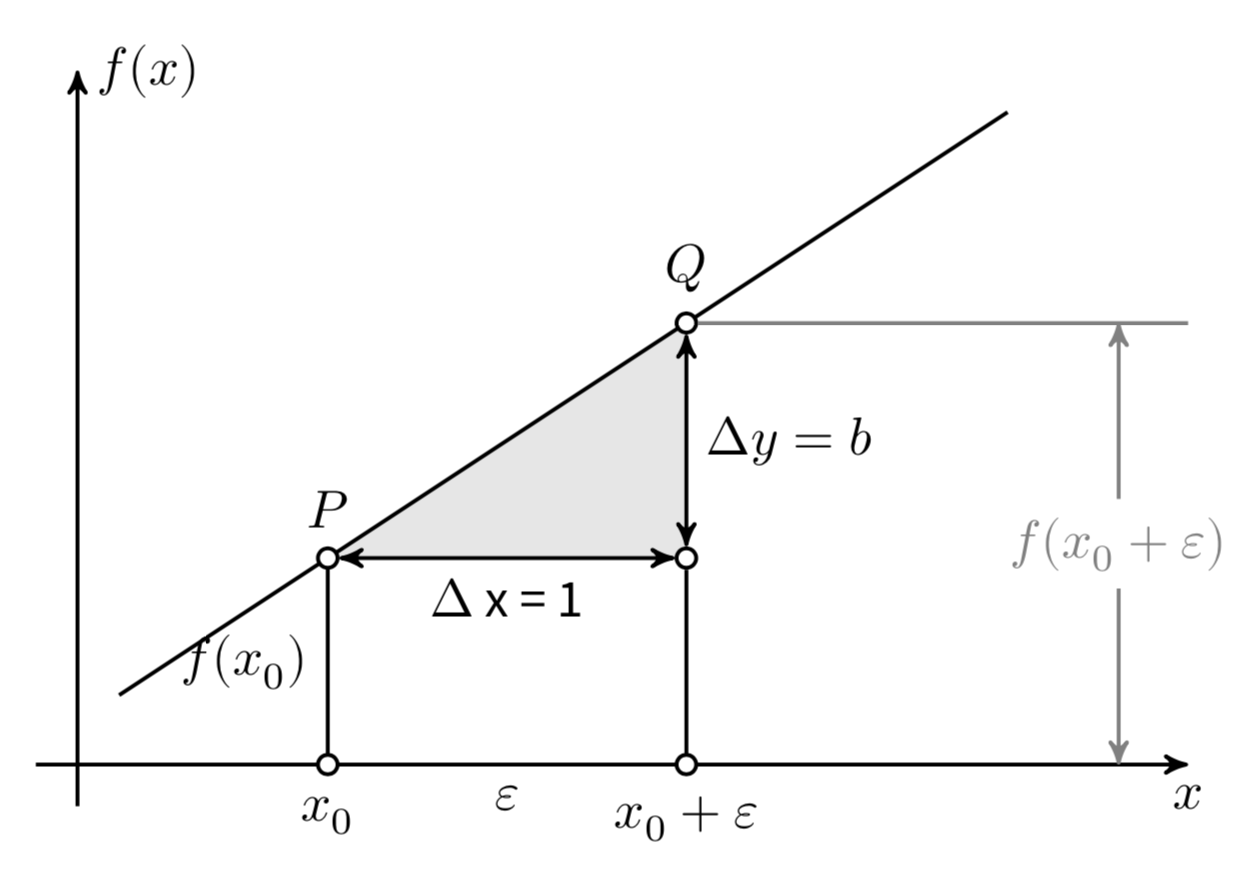
\includegraphics[width=0.7\linewidth]{images/linear_function} 

}

\caption{La funzione lineare $y = a + bx$.}\label{fig:linearfunction}
\end{figure}

\hypertarget{lerrore-di-misurazione}{%
\section{L'errore di misurazione}\label{lerrore-di-misurazione}}

Per descrivere l'associazione tra due variabili, tuttavia, la funzione lineare non è sufficiente. Nel mondo empirico, infatti, la relazione tra variabili non è mai perfettamente lineare. È dunque necessario includere nel modello di regressione anche una componente d'errore, ovvero una componente della \(y\) che non può essere spiegata dal modello lineare. Nel caso di due sole variabili, questo ci conduce alla seguente formulazione del modello di regressione:

\begin{equation}
y = \alpha + \beta x + \varepsilon,
\label{eq:regbivpop}
\end{equation}

laddove i parametri \(\alpha\) e \(\beta\) descrivono l'associazione tra le variabili casuali \(y\) e \(x\), e il termine d'errore \(\varepsilon\) specifica quant'è grande la porzione della variabile \(y\) che non può essere predetta nei termini di una relazione lineare con la \(x\).

Si noti che la \eqref{eq:regbivpop} consente di formulare una predizione, nei termini di un modello lineare, del valore atteso della \(y\) conoscendo \(x\), ovvero

\begin{equation}
\hat{y} = \mathbb{E}(y \mid x) = \alpha + \beta x.
\label{eq:regbivpop2}
\end{equation}

In altri termini, se i parametri del modello (\(\alpha\) e \(\beta\)) sono noti, allora è possibile predire la \(y\) sulla base della nostra conoscenza della \(x\).
Per esempio, se conosciamo la relazione lineare tra quoziente di intelligenza ed aspettativa di vita, allora possiamo prevedere quanto a lungo vivrà una persona sulla base del suo QI. Sì, c'è una relazione lineare tra intelligenza e aspettativa di vita \autocite{hambrick2015research}! Ma quando è accurata la previsione? Ciò dipende dal termine d'errore della \eqref{eq:regbivpop}. L'analisi di regressione fornisce un metodo per rispondere a domande di questo tipo\footnote{Per una discussione sugli aspetti di base della regressione lineare, si veda il \href{https://openintro-ims.netlify.app/model-slr.html}{capitolo 7} di \emph{Introduction to Modern Statistics}.}.

\hypertarget{una-media-per-ciascuna-osservazione}{%
\section{Una media per ciascuna osservazione}\label{una-media-per-ciascuna-osservazione}}

In precedenza abbiamo visto come sia possibile stimare i parametri di un modello bayesiano Normale nel quale le osservazioni sono indipendenti e identicamente distribuite secondo una densità Normale,
\begin{equation}
Y_i \stackrel{i.i.d.}{\sim} \mathcal{N}(\mu, \sigma), \quad i = 1, \dots, n.
\label{eq:normalsamplingmodel}
\end{equation}

Il modello \eqref{eq:normalsamplingmodel} assume che ogni \(Y_i\) sia una realizzazione della stessa \(\mathcal{N}(\mu, \sigma^2)\). Da un punto di vista bayesiano\footnote{Per un'introduzione alla trattazione frequentista dell'analisi di regressione, si veda l'Appendice \ref{least-squares}.}, si assegnano distribuzioni a priori ai parametri \(\mu\) e \(\sigma\), si genera la verosimiglianza in base ai dati osservati e, con queste informazioni, si generano le distribuzione a posteriori dei parametri \autocite{gelman2020regression}:
\begin{align}
Y_i \mid \mu, \sigma & \stackrel{iid}{\sim} \mathcal{N}(\mu, \sigma^2)\notag\\
\mu       & \sim \mathcal{N}(\mu_0, \tau^2) \notag\\
\sigma    & \sim \Cauchy(x_0, \gamma) \notag
\end{align}

È comune però che vengano però registrate altre variabili \(x_i\) che possono essere associate alla risposta di interesse \(y_i\). La variabile \(x_i\) viene chiamata \emph{predittore} (o variabile indipendente) in quanto il ricercatore è tipicamente interessato a predire il valore \(y_i\) a partire da \(x_i\). Come si può estende il modello Normale della \eqref{eq:normalsamplingmodel} per lo studio della possibile relazione tra \(y_i\) e \(x_i\)?

Il modello \eqref{eq:normalsamplingmodel} assume una media \(\mu\) comune per ciascuna osservazione \(Y_i\). Dal momento che desideriamo introdurre una nuova variabile \(x_i\) che assume un valore specifico per ciascuna osservazione \(y_i\), il modello \eqref{eq:normalsamplingmodel} può essere modificato in modo che la media comune \(\mu\) venga sostituita da una media \(\mu_i\) specifica a ciascuna \(i\)-esima osservazione:

\begin{equation}
Y_i \mid \mu_i, \sigma \stackrel{ind}{\sim} \mathcal{N}(\mu_i, \sigma), \quad i = 1, \dots, n.
\label{eq:normalsamplinglinearmodel}
\end{equation}

Si noti che le osservazioni \(Y_1, \dots, Y_n\) non sono più identicamente distribuite poiché hanno medie diverse, ma sono ancora indipendenti come indicato dalla notazione \texttt{ind} posta sopra il simbolo \(\sim\) nella \eqref{eq:normalsamplinglinearmodel}

\hypertarget{relazione-lineare-tra-la-media-e-il-predittore}{%
\subsection{Relazione lineare tra la media e il predittore}\label{relazione-lineare-tra-la-media-e-il-predittore}}

L'approccio che consente di mettere in relazione un predittore \(x_i\) con la risposta \(Y_i\) è quello di assumere che la media di ciascuna \(Y_i\), ovvero \(\mu_i\), sia una funzione lineare del predittore \(x_i\). Una tale relazione lineare è scritta come

\begin{equation}
\mu_i = \beta_0 + \beta_ 1 x_i, \quad i = 1, \dots, n.
\label{eq:regmodel}
\end{equation}

Nella \eqref{eq:regmodel}, ciascuna \(x_i\) è una costante nota (ecco perché viene usata una lettera minuscola per la \(x\)) e \(\beta_0\) e \(\beta_ 1\) sono parametri incogniti. Questi parametri che rappresentano l'intercetta e la pendenza della retta di regressione sono variabili casuali. Si assegna una distribuzione a priori a \(\beta_0\) e a \(\beta_ 1\) e si esegue l'inferenza riassumendo la distribuzione a posteriori di questi parametri.

In questo modello, la funzione lineare \(\beta_0 + \beta_ 1 x_i\) è interpretata come il valore atteso della \(Y_i\) per ciascun valore \(x_i\), mentre l'intercetta \(\beta_0\) rappresenta il valore atteso della \(Y_i\) quando \(x_i = 0\). Il parametro \(\beta_ 1\) (pendenza) rappresenta invece l'aumento medio della \(Y_i\) quando \(x_i\) aumenta di un'unità. È importante notare che la relazione lineare \eqref{eq:normalsamplinglinearmodel} di parametri \(\beta_0\) e \(\beta_ 1\) descrive l'associazione tra \emph{la media} \(\mu_i\) e il predittore \(x_i\). In altri termini, tale relazione lineare ci fornisce una predizione sul valore medio \(\mu_i\), non sul valore \emph{effettivo} \(Y_i\).

\hypertarget{il-modello-di-regressione-lineare}{%
\subsection{Il modello di regressione lineare}\label{il-modello-di-regressione-lineare}}

Sostituendo la \eqref{eq:regmodel} nel modello \eqref{eq:normalsamplinglinearmodel} otteniamo il modello di regressione lineare:

\begin{equation}
Y_i \mid \beta_0, \beta_ 1, \sigma \stackrel{ind}{\sim} \mathcal{N}(\beta_0 + \beta_ 1 x_i, \sigma), \quad i = 1, \dots, n.
\label{eq:samplinglinearmodel}
\end{equation}

Questo è un caso speciale del modello di campionamento Normale, dove le \(Y_i\) seguono indipendentemente una densità Normale con una media (\(\beta_0 + \beta_ 1 x_i\)) specifica per ciascuna osservazione e con una deviazione standard (\(\sigma\)) comune a tutte le osservazioni. Poiché include un solo predittore (\(x\)), questo modello è comunemente chiamato \emph{modello di regressione lineare semplice}.

In maniera equivalente, il modello \eqref{eq:samplinglinearmodel} può essere formulato come

\begin{equation}
Y_i = \mu_i + \varepsilon_i, \quad i = 1, \dots, n,
\label{eq:samplinglinearmodel2}
\end{equation}

dove la risposta media è \(\mu_i = \beta_0 + \beta_ 1 x_i\) e i residui \(\varepsilon_1, \dots, \varepsilon_n\) sono i.i.d. da una Normale con media 0 e deviazione standard \(\sigma\).

\begin{center}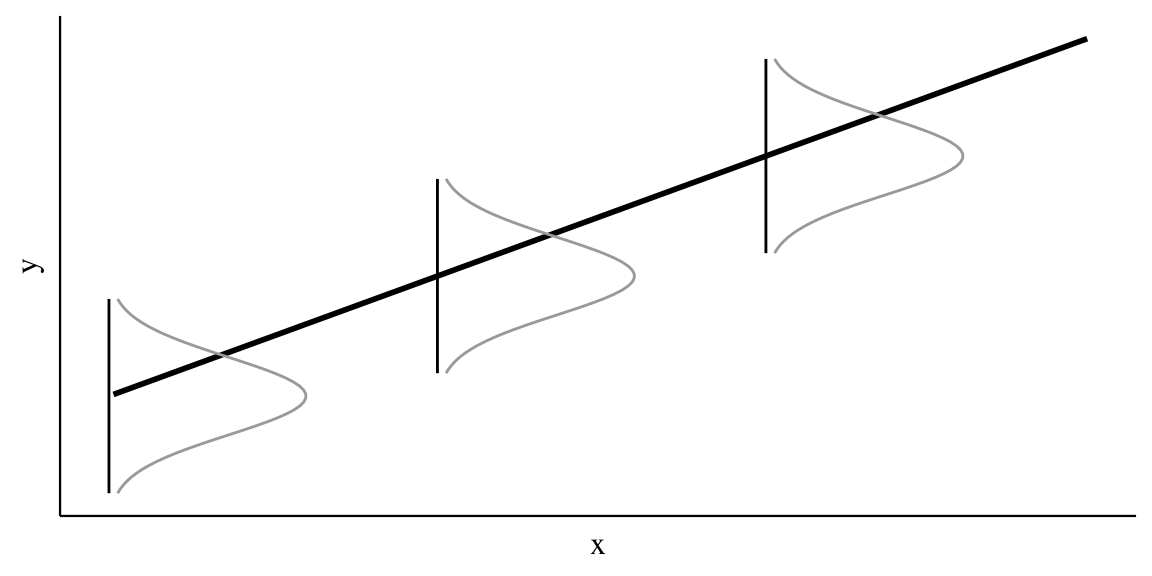
\includegraphics[width=0.8\linewidth]{051_reglin1_files/figure-latex/unnamed-chunk-2-1} \end{center}

Nel modello di regressione lineare, l'osservazione \(Y_i\) è una variabile casuale, il predittore \(x_i\) è una costante fissa, e \(\beta_0\), \(\beta_1\) e \(\sigma\) sono parametri incogniti. Utilizzando il paradigma bayesiano, viene assegnata una distribuzione a priori congiunta a \((\beta_0, \beta_1, \sigma)\). Dopo avere osservato le risposte \(Y_i, i = 1, \dots, n\), l'inferenza procede stimando la distribuzione a posteriori dei parametri.

Nella costruzione di un modello di regressione bayesiano, è importante iniziare dalle basi e procedere un passo alla volta. Sia \(Y\) una variabile di risposta e
sia \(x\) un predittore o un insieme di predittori. È possibile costruire un modello di regressione di \(Y\) su \(x\) applicando i seguenti principi generali:

\begin{itemize}
\tightlist
\item
  Stabilire se \(Y\) è discreto o continuo. Di conseguenza, identificare l'appropriata struttura dei dati (per esempio, Normale, di Poisson, o Binomiale).
\item
  Esprimere la media di \(Y\) come funzione dei predittori \(x\) (per esempio, \(\mu = \beta_0 + \beta_1 x\)).
\item
  Identificare tutti i parametri incogniti del modello (per esempio, \(\mu, \beta_1, \beta_2\)).
\item
  Valutare quali valori che ciascuno di questi parametri potrebbe assumere. Di conseguenza, identificare le distribuzioni a priori appropriate per questi parametri.
\end{itemize}

Nel caso di una variabile \(Y\) continua che segue la legge Normale e un solo predittore, ad esempio, il modello diventa:

\begin{align} 
Y_i \mid \beta_0, \beta_1, \sigma  &\stackrel{ind}{\sim} \mathcal{N}\left(\mu_i, \sigma^2\right) \;\; \text{ con } \;\; \mu_i = \beta_0 + \beta_1 x_i \notag\\
\beta_0  &\sim \mathcal{N}\left(\mu_0, \sigma_0^2 \right)  \notag\\
\beta_1  & \sim \mathcal{N}\left(\mu_1, \sigma_1^2 \right) \notag\\
\sigma & \sim \text{Cauchy}(x_0, \gamma) \; .\notag
\end{align}

Un algoritmo MCMC viene usato per simulare i campioni dalle distribuzioni a posteriori e, mediante tali campioni, si fanno inferenze sulla risposta attesa \(\beta_0 + \beta_1 x\) per ciascuno specifico valore del predittore \(x\). Inoltre, è possibile valutare le dimensioni degli errori di previsione mediante un indice sintetico della densità a posteriori della deviazione standard \(\sigma\).

\hypertarget{considerazioni-conclusive}{%
\section*{Considerazioni conclusive}\label{considerazioni-conclusive}}
\addcontentsline{toc}{section}{Considerazioni conclusive}

Il modello di regressione lineare semplice viene usato per descrivere la
relazione tra due variabili e per determinare il segno e l'intensità di
tale relazione. Inoltre, il modello di regressione ci consente di
prevedere il valore della variabile dipendente in base ad alcuni nuovi
valori della variabile indipendente. Il modello di regressione lineare
semplice è in realtà molto limitato, in quanto descrive soltanto la
relazione tra la variabile dipendente \(y\) e una sola variabile
esplicativa \(x\). Esso diventa molto più utile quando incorpora più
variabili indipendenti. In questo secondo caso, però, i calcoli per la
stima dei coefficienti del modello diventano più complicati. Abbiamo
deciso di iniziare considerando il modello di regressione lineare semplice
perché, in questo caso, sia la logica dell'inferenza sia le procedure di
calcolo sono facilmente maneggiabili. Nel caso più generale, quello del
modello di regressione multipla, la logica dell'inferenza rimarrà
identica a quella discussa qui, ma le procedure di calcolo richiedono
l'uso dell'algebra matriciale. Il modello di regressione multipla può includere sia regressori quantitativi, sia regressori qualitativi, utilizzando un
opportuna schema di codifica. È interessante notare come un modello di
regressione multipla che include una sola variabile esplicativa
quantitativa corrisponde all'analisi della varianza ad una via; un
modello di regressione multipla che include più di una variabile
esplicativa quantitativa corrisponde all'analisi della varianza più vie.
Possiamo qui concludere dicendo che il modello di regressione, nelle sue varie forme e varianti, costituisce la tecnica di analisi dei dati maggiormente usata in psicologia.


% Bibliography
%%%%%%%%%%%%%%%%%%%%%%%%%%%%%%%%%%%%%%%%%%%%%%%%%%%%%%%%%%

\backmatter
\SmallMargins

\printbibliography
\onecolumn


% Tables (of tables, of figures)
%%%%%%%%%%%%%%%%%%%%%%%%%%%%%%%%%%%%%%%%%%%%%%%%%%%%%%%%%%


\cleardoublepage
\LargeMargins
\listoffigures


% After-body (LaTeX code inclusion)
%%%%%%%%%%%%%%%%%%%%%%%%%%%%%%%%%%%%%%%%%%%%%%%%%%%%%%%%%%




% Back cover
%%%%%%%%%%%%%%%%%%%%%%%%%%%%%%%%%%%%%%%%%%%%%%%%%%%%%%%%%%%

% Even page, small margins, no running head, no page number.
\evenpage
\SmallMargins
\thispagestyle{empty}

\begin{normalsize}

\begin{description}

\selectlanguage{italian}
\item[Abstract]
This document contains the material of the lessons of Psicometria B000286 (2021/2022) aimed at students of the first year of the Degree Course in Psychological Sciences and Techniques of the University of Florence, Italy.
\item[Keywords]
Data science, Bayesian statistics.
~\\

\end{description}

\end{normalsize}


\end{document}
